\documentclass[class=jsarticle, crop=false, dvipdfmx, fleqn]{standalone}
%% preamble for Numerical-structure-analysis report

\input{/Users/User/Documents/Project/TeX/preamble/mypreamble}

%% titles
\title{先端データ解析論 レポート}
\author{37-196360 \quad 森田涼介}


%% setting for listings
\newtcbinputlisting[auto counter]{\reportlisting}[3][]{%
	listing file = {#3},
	listing options = {language=python, style=tcblatex, numbers=left, numberstyle=\tiny},
	listing only,
	breakable,
	toprule at break = 0mm,
	bottomrule at break = 0mm,
	left = 6mm,
	sharp corners,
	drop shadow,
	title = Listings \thetcbcounter : \texttt{#2},
	label = #1,
	}



%% title format
\usepackage{titlesec}
\titleformat{\section}{\LARGE}{宿題\thesection}{0zw}{}
\newcommand{\sectionbreak}{\clearpage}
\titleformat{\subsection}{\Large}{\Alph{subsection})}{0zw}{}

\begin{document}
\section{}

ガウスカーネルモデルに対するL2正則化を用いた最小二乗回帰の交差確認法を実装し,
正則化パラメータとガウス幅を決定する。

ガウスカーネルモデルは次のように表される。
\begin{align}
	& f_{\bm{\theta}} (\bm{x}) = \sum_{j=1}^{n} \theta_j K(\bm{x},\ \bm{x}_j) \\
	& K(\bm{x}, \bm{c}) = \exp(-\frac{||\bm{x} - \bm{c}||^2}{2 h^2})
\end{align}
このとき,L2正則化を用いた最小二乗誤差は,
\begin{align}
	& L(\bm{\theta}) = \frac{1}{2} ||\bm{K \theta} - \bm{y}||^2 + \frac{\lambda}{2} ||\bm{\theta}||^2 \\
	& \bm{K} =
		\begin{bmatrix}
			K(\bm{x}_1,\ \bm{x}_1) & \cdots & K(\bm{x}_1,\ \bm{x}_n) \\
			\vdots & \ddots & \vdots \\
			K(\bm{x}_n,\ \bm{x}_1) & \cdots & K(\bm{x}_n,\ \bm{x}_n)
		\end{bmatrix}
\end{align}
と表される。
ここで,$L$の$\bm{\theta}$による偏微分が$\bm{0}$となるような$\bm{\theta} = \hat{\bm{\theta}}$が$L$に最小値を与えることから,
\begin{align}
	\pdv{L}{\bm{\theta}}
		& = \bm{K}^\mathrm{T} \bm{K \theta} - \bm{K}^\mathrm{T} \bm{y} + \lambda \bm{\theta} \\
		& = (\bm{K}^2 + \lambda \bm{I}) \bm{\theta} - \bm{K y} \\
	\hat{\bm{\theta}} & = (\bm{K}^2 + \lambda \bm{I})^{-1} \bm{K y}
\end{align}
ここで,$\bm{K}$が対称行列であることを用いた。

いま,真のデータが
\begin{equation}
	f(x) = \sin(\pi x) / (\pi x) + 0.1 x
		\quad (-3 \leq x < 3 )
\end{equation}
から生成されていて,
そのサンプルが50個ある場合を考える。
このデータに対しガウスカーネルモデルを適用し,
交差確認法によってそのハイパーパラメータ$h,\ \lambda$を推定する。
いま,交差確認法のために,データを5分割し,
それぞれのテスト誤差の平均をそのモデルのテスト誤差とした。
また,テスト誤差にはL2正則化項は含まず,$y$の推定値と真の値の二乗和誤差のみを用いた。

まず,大域的に探索するため,
\begin{align}
	& h = \num{1e-2},\ \num{1e-1},\ \num{1},\ \num{1e1} \\
	& \lambda = \num{1e-6},\ \num{1e-5},\ \num{1e-4},\ \num{1e-3},\ \num{1e-2},\ \num{1e-1}
\end{align}
として,各$(h,\ \lambda)$の組について交差確認法を用いて誤差を計算したところ,
\begin{align}
	& h = 1 \\
	& \lambda = \num{1e-5} \\
	& L = 1.106
\end{align}
と求まった。
次に,求まった範囲の付近で最適なものを探したところ,
\begin{align}
	& h = 1.1 \\
	& \lambda = \num{8e-7} \\
	& L = 1.04
\end{align}
と求まった。

大域的に探索したときの結果を図\ref{fig:result_global_search}に示す。
これより,ガウス幅は0.1--1.0あたりに設定する必要があることがわかる。
また,プログラムは\pageref{listing:assignment1}ページのListing \ref{listing:assignment1}に記載した。

\begin{figure}
	\centering
	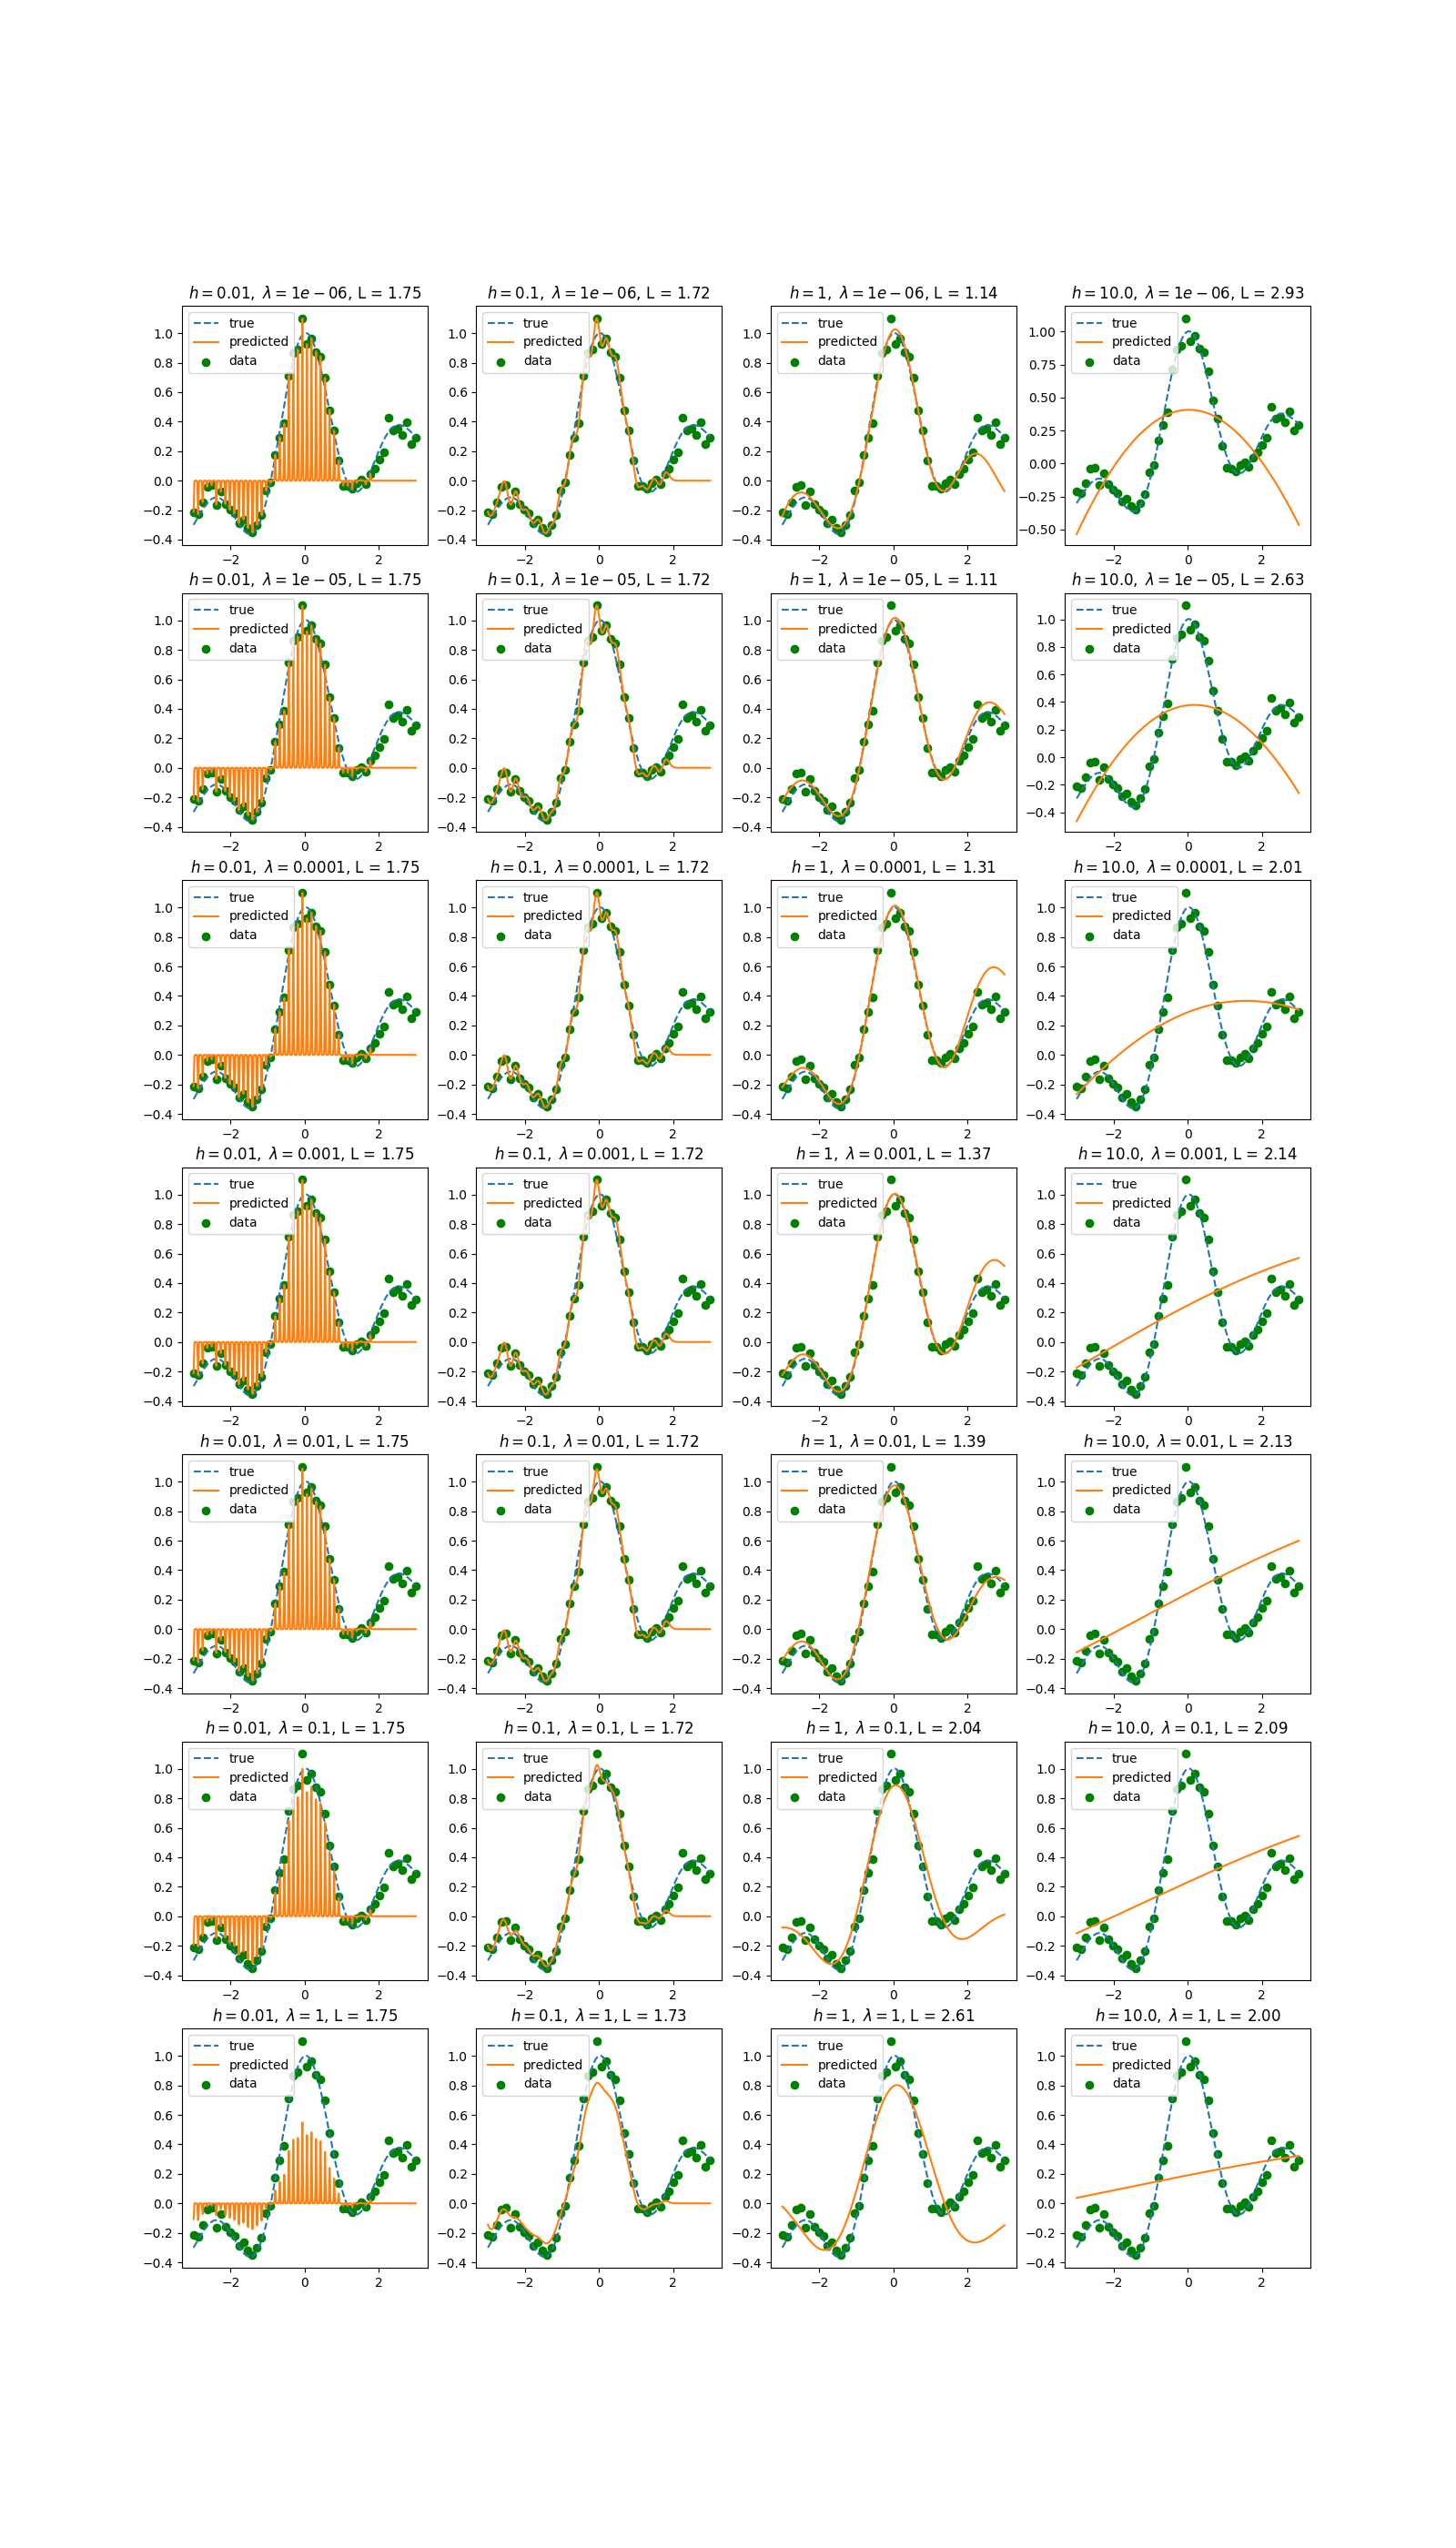
\includegraphics[clip, width=15cm, trim=0 144 0 216]{../figures/assignment1_result}
	\caption{交差確認法の結果}
	\label{fig:result_global_search}
\end{figure}


\end{document}